% !TEX encoding = UTF-8
\chapter{Tổng quan}

\section{Đặt vấn đề}

\subsection{Hạn chế của mô hình bảo mật dựa trên vành đai trong kiến trúc Microservices}

Trong nhiều thập kỷ, an toàn thông tin doanh nghiệp được xây dựng dựa trên mô hình phòng thủ chu vi (perimeter-based defense), hay còn gọi là chiến lược ``lâu đài và hào nước'' \cite[tr. 5]{gilman2017zero}. Mô hình này thiết lập ranh giới rõ ràng giữa mạng nội bộ được tin cậy và thế giới Internet bên ngoài thông qua tường lửa và VPN. Bất kỳ thực thể nào vượt qua được vành đai này đều được ngầm định trao cho sự tin cậy rất lớn để di chuyển bên trong mạng. 

Tuy nhiên, sự dịch chuyển từ các ứng dụng nguyên khối (Monolithic) sang kiến trúc vi dịch vụ (Microservices) đã làm ranh giới vật lý tĩnh này biến mất hoàn toàn. Việc chia nhỏ ứng dụng thành hàng trăm dịch vụ phân tán thay thế các lệnh gọi hàm nội bộ bằng các lệnh gọi qua mạng, từ đó tạo ra bề mặt tấn công rộng lớn. Một khi tin tặc vượt qua được vành đai bảo vệ bên ngoài, sự tin tưởng ngầm định của mô hình cũ cho phép chúng dễ dàng thực hiện dịch chuyển ngang (\textit{Lateral Movement}), leo thang đặc quyền và tiếp cận các tài sản quan trọng mà không gặp phải rào cản nào \cite[tr. 12]{rose2020zero}.

\begin{figure}[H]
    \centering
    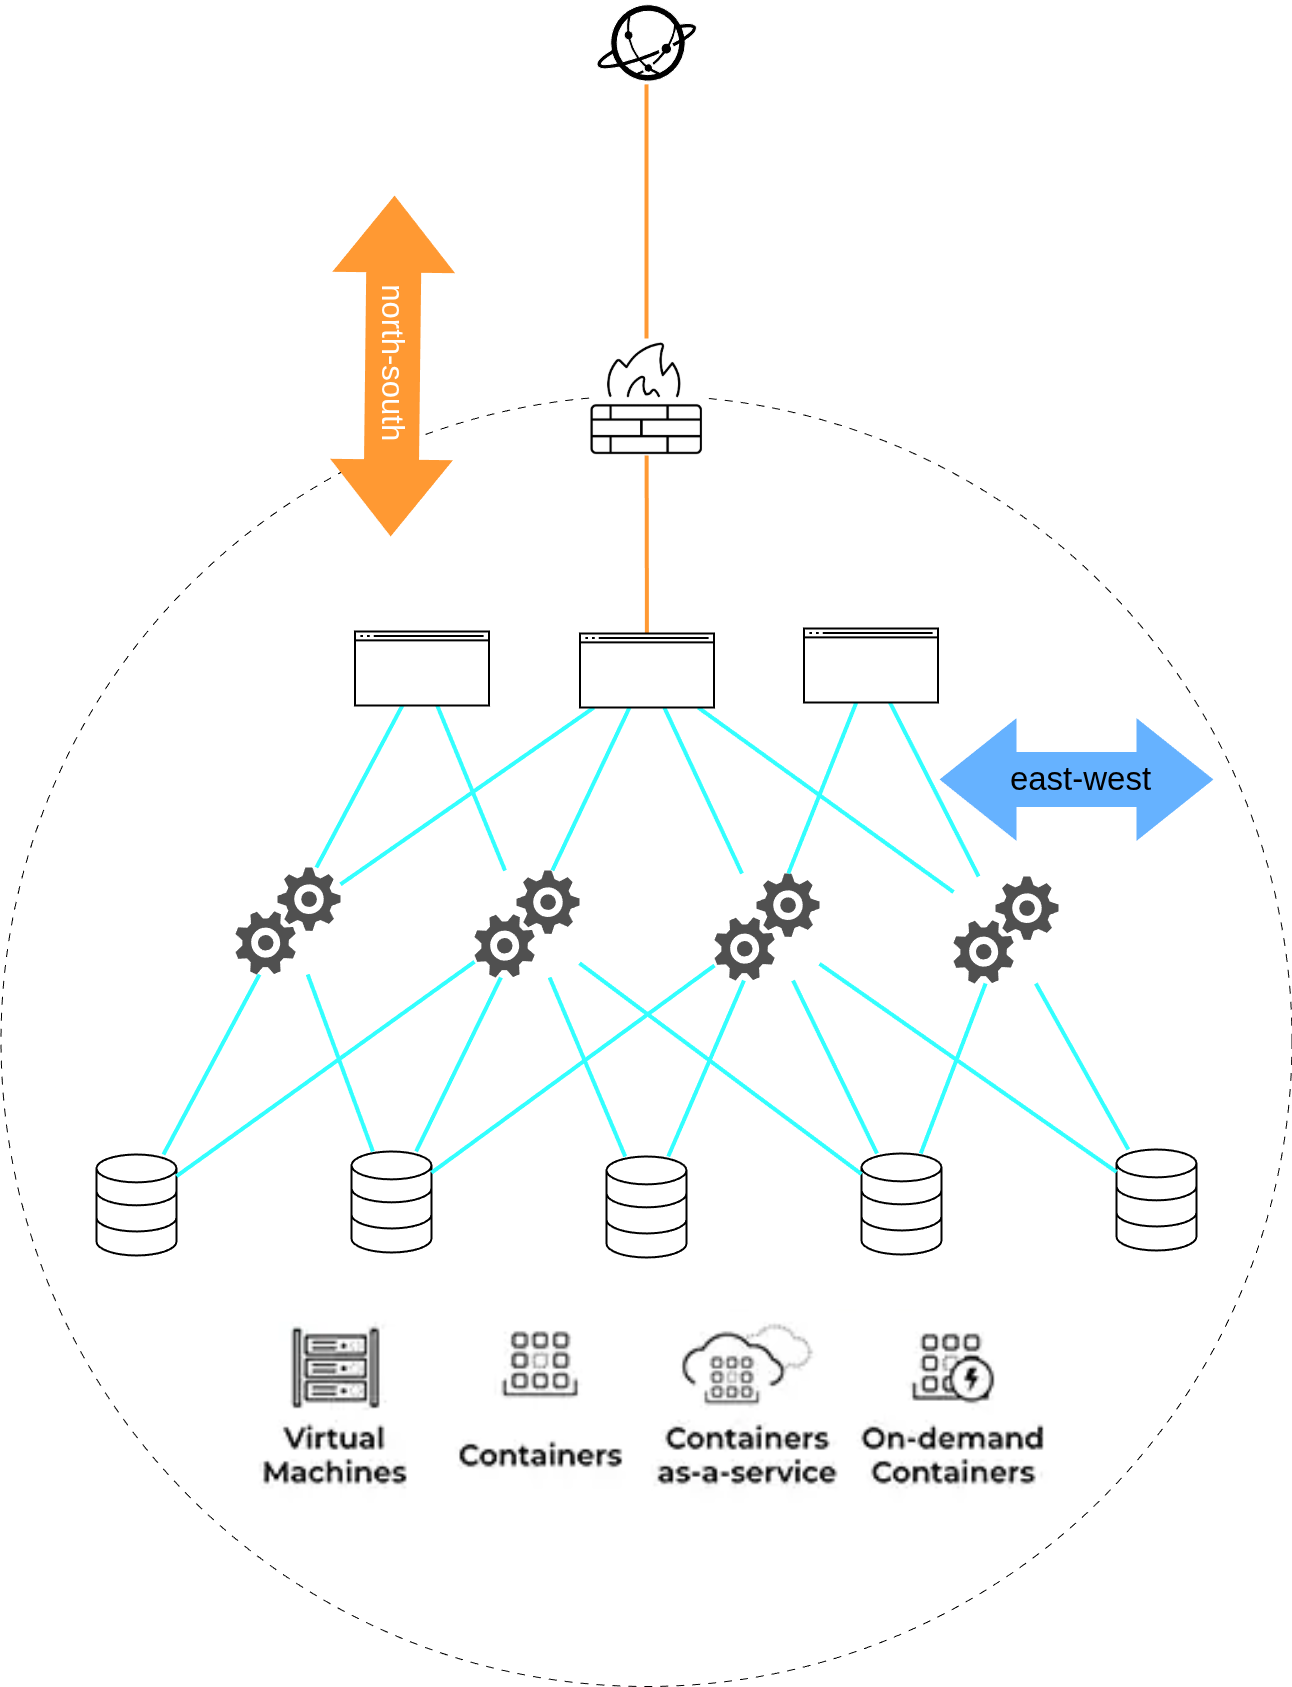
\includegraphics[height=0.8\textheight]{images/nsew.png}
    \caption{Lưu lượng \textit{North-South} (từ Internet vào hệ thống) và \textit{East-West} (giữa các dịch vụ nội bộ)}
    \label{fig:nsew}
\end{figure}

\newpage

\subsection{Các thách thức bảo mật đặc thù của môi trường Kubernetes}

Kubernetes là nền tảng điều phối container tiêu chuẩn, nhưng nó cũng mang lại những thách thức an ninh phức tạp. Môi trường này chứa các thực thể phù du (như \textit{Pod}) có vòng đời rất ngắn, bị xóa sổ và tạo mới liên tục với các địa chỉ IP thay đổi linh hoạt \cite{rice2019kubernetes}. Do đó, việc áp dụng các chính sách bảo mật dựa trên địa chỉ IP tĩnh như mô hình vành đai truyền thống trở nên vô dụng. 

Bên cạnh đó, số lượng danh tính phi con người (\textit{Machine Identities, Workloads, Service Accounts}) giao tiếp với nhau (lưu lượng \textit{East-West}) áp đảo danh tính con người, tạo ra bài toán hóc búa về việc quản lý chuỗi bí mật (\textit{Secret Zero problem}). Nếu không có sự phân đoạn mạng vi mô (\textit{Micro-segmentation}), một container bị chiếm quyền điều khiển có thể trở thành bàn đạp để kẻ tấn công quét mạng và thâm nhập vào các vi dịch vụ trọng yếu khác đang chạy chung trên cùng một cụm.



\subsection{Mục tiêu và phạm vi nghiên cứu}

Nhằm giải quyết những hạn chế của mô hình bảo mật cũ trong kiến trúc phân tán, mục tiêu của nghiên cứu là thiết kế và triển khai \textbf{Kiến trúc Zero Trust (ZTA)} để bảo vệ toàn diện hệ thống Microservices trên môi trường Kubernetes. Phạm vi nghiên cứu tập trung vào:
\begin{itemize}
    \item Áp dụng các công nghệ hiện đại như \textbf{eBPF} (thông qua \textit{Cilium} và \textit{Tetragon} \cite{cilium_docs}) để kiểm soát truy cập tầng mạng và giám sát an ninh tại thời gian thực (\textit{Runtime Security}) mà không làm suy giảm hiệu năng.
    \item Tích hợp \textit{Identity Provider} làm điểm quản trị chính sách xác thực, kết hợp triển khai \textbf{mTLS (Mutual TLS)} nhằm xác thực danh tính hai chiều giữa các dịch vụ.
    \item Xây dựng luồng (pipeline) giám sát và cảnh báo an ninh tập trung (\textit{Observability}) bằng ELK Stack, Prometheus và Grafana.
\end{itemize}

\newpage

\section{Tổng quan về Kiến trúc Zero Trust (ZTA)}

\subsection{Lịch sử hình thành và động lực ra đời}

Khái niệm ``Zero Trust'' (Không tin cậy) lần đầu tiên được định hình bởi nhà phân tích John Kindervag vào năm 2010 khi ông làm việc tại Forrester Research \cite{kindervag2010build}, mặc dù những ý tưởng nền tảng về giải trừ chu vi (\textit{de-perimeterization}) đã được Jericho Forum đề cập từ năm 2004 \cite{jericho2004}. 

Động lực chính dẫn đến sự ra đời của Zero Trust là sự bùng nổ của điện toán đám mây, ứng dụng SaaS và xu hướng làm việc từ xa, khiến ranh giới mạng nội bộ doanh nghiệp không còn tồn tại. Việc phụ thuộc vào ``sự tin cậy ngầm định'' đã tạo điều kiện cho các chiến thuật tấn công dịch chuyển ngang gây ra những vụ rò rỉ dữ liệu thảm khốc. Do đó, Zero Trust ra đời với triết lý cốt lõi: \textit{“Không bao giờ tin cậy, luôn luôn xác minh” (Never trust, always verify)}, yêu cầu mọi kết nối đều phải bị coi là thù địch cho đến khi được xác thực rõ ràng.

% !TEX encoding = UTF-8

\subsection{Các nguyên lý cốt lõi theo NIST SP 800-207}

Viện Tiêu chuẩn và Công nghệ Quốc gia Hoa Kỳ (NIST) đã hệ thống hóa ZTA thông qua ấn phẩm NIST SP 800-207 \cite{rose2020zero} với 7 nguyên lý trọng tâm. Trọng tâm của mô hình này là đặt tài nguyên lên hàng đầu (\textit{Resource-First Security}), cụ thể:

\begin{itemize}
    \item \textbf{Mọi nguồn dữ liệu và dịch vụ điện toán đều là tài nguyên:} \\
    Phạm vi bảo vệ không chỉ dừng lại ở máy chủ vật lý mà bao trùm mọi thiết bị, dịch vụ đám mây (SaaS), vi dịch vụ (Microservices) và hệ thống API. \\
    Ví dụ: Một cổng thông tin nhân sự nội bộ (SaaS) và một API truy vấn cơ sở dữ liệu backend đều được hệ thống ZTA định danh là hai tài nguyên độc lập. Chúng yêu cầu các chính sách kiểm soát quyền truy cập riêng biệt thay vì chỉ được bảo vệ chung bởi một mạng riêng ảo (VPN).

    \item \textbf{Mọi giao tiếp đều phải được bảo mật bất kể vị trí mạng:} \\
    Hệ thống loại bỏ hoàn toàn khái niệm ``vùng tin cậy ẩn'' (\textit{implicit trust zone}). Mọi kết nối nội bộ (trong cùng một trung tâm dữ liệu) hay từ Internet đều phải được mã hóa và xác thực. \\
    Ví dụ: Trong cụm Kubernetes, mặc dù vi dịch vụ \texttt{OrderService} và \texttt{PaymentService} nằm trên cùng một Node nội bộ, lưu lượng giao tiếp giữa chúng vẫn bắt buộc phải được mã hóa và xác thực danh tính hai chiều bằng chứng chỉ số (mTLS) để phòng ngừa bị nghe lén nếu mạng nội bộ bị xâm nhập.

    \item \textbf{Quyền truy cập được cấp trên cơ sở từng phiên làm việc (per-session):} \\
    Tuân thủ nghiêm ngặt nguyên tắc đặc quyền tối thiểu (\textit{Least Privilege}). Sự tin cậy được đánh giá trước khi kết nối và hệ thống chỉ cấp quyền vừa đủ để chủ thể thực hiện một tác vụ cụ thể, sau đó thu hồi ngay. \\
    Ví dụ : Một người dùng được cấp quyền ``Chỉ đọc'' (Read-only) để xem báo cáo tài chính. Nếu người này cố gắng thực hiện lệnh ``Xóa'' (Delete) hoặc chuyển sang xem một tài liệu khác, hệ thống sẽ yêu cầu đánh giá lại quyền hạn cho phiên làm việc mới đó thay vì tiếp tục tin tưởng.

    \item \textbf{Quyền truy cập được xác định bởi chính sách động (dynamic policy):} \\
    Quyết định cấp quyền không dựa trên các quy tắc tĩnh (như dải địa chỉ IP) mà dựa trên việc tổng hợp nhiều tín hiệu ngữ cảnh: danh tính, trạng thái thiết bị, hành vi lịch sử, và vị trí địa lý. \\
    Ví dụ: Một lập trình viên có thể truy cập vào mã nguồn của công ty từ laptop được cấp phát khi đang ngồi tại văn phòng. Tuy nhiên, nếu lập trình viên đó dùng chính tài khoản này nhưng đăng nhập từ mạng Wi-Fi công cộng tại quán cà phê hoặc trên một thiết bị cá nhân không được quản lý, hệ thống động (Policy Engine) sẽ lập tức từ chối truy cập.
    
    \item \textbf{Giám sát và đo lường tính toàn vẹn của mọi tài sản:} \\
    Tổ chức phải liên tục đánh giá trạng thái an ninh của thiết bị. Truy cập sẽ bị từ chối nếu thiết bị có dấu hiệu bị thỏa hiệp hoặc không tuân thủ chính sách bảo mật. \\
    Ví dụ: Hệ thống quản lý thiết bị (MDM) phát hiện laptop của nhân viên chưa cập nhật bản vá lỗ hổng hệ điều hành mới nhất hoặc phần mềm diệt virus đã bị tắt. Ngay lập tức, thiết bị này bị tước quyền truy cập vào các ứng dụng nội bộ cho đến khi hoàn tất việc cập nhật.
    
    \item \textbf{Xác thực và ủy quyền phải linh hoạt và thực thi nghiêm ngặt trước khi truy cập:} \\
    Không chỉ xác thực một lần ở đầu phiên, hệ thống áp dụng xác thực đa yếu tố (MFA) và liên tục tái xác thực (\textit{continuous re-authentication}) trong suốt vòng đời của phiên kết nối. \\
    Ví dụ: Quản trị viên hệ thống đám mây đã đăng nhập thành công vào AWS Console được 2 giờ. Tuy nhiên, khi người này thực hiện một hành động nhạy cảm cao như xóa một \textit{S3 Bucket} chứa dữ liệu người dùng, hệ thống bắt buộc họ phải cắm khóa bảo mật vật lý (YubiKey) hoặc nhập mã sinh trắc học để xác thực lại một lần nữa.

    \item \textbf{Thu thập tối đa thông tin tình báo, nhật ký (Telemetry and Logs):} \\
    Dữ liệu đo từ xa về mạng, thiết bị và hành vi được sử dụng để phân tích, cải thiện tư thế bảo mật và tự động tinh chỉnh chính sách theo thời gian thực. \\
    Ví dụ: Nền tảng phân tích an ninh (SIEM) thu thập nhật ký truy cập và dùng học máy (Machine Learning) để phát hiện một tài khoản nhân sự đột nhiên tải xuống 1.000 hồ sơ ứng viên lúc 2 giờ sáng. Hệ thống tự động kích hoạt kịch bản phản ứng: khóa tạm thời tài khoản và gửi cảnh báo đỏ cho đội ngũ vận hành bảo mật (SOC).
\end{itemize}

\subsection{Năm trụ cột chức năng cốt lõi theo Mô hình CISA ZTMM 2.0}

Để hiện thực hóa 7 nguyên tắc của NIST vào thực tiễn tổ chức, Cơ quan An ninh Mạng và Cơ sở Hạ tầng Hoa Kỳ (CISA) đã phát hành \textit{Mô hình Trưởng thành Zero Trust (ZTMM) phiên bản 2.0} \cite{cisa_ztmm2023}. Mô hình này chia kiến trúc Zero Trust thành 5 trụ cột cấu thành những lĩnh vực bảo vệ thiết yếu, được hỗ trợ bởi 3 năng lực xuyên suốt:

\begin{itemize}
    \item \textbf{Danh tính (Identity):} \\
    Đảm bảo chỉ những người dùng hợp lệ và các thực thể phi nhân sự (máy móc, dịch vụ) mới có quyền truy cập. Yêu cầu thực thi MFA toàn diện và loại bỏ các đặc quyền thường trực (Standing privileges) thông qua cơ chế cấp quyền ``đúng lúc'' (\textit{Just-In-Time - JIT}). \\
    Ví dụ: Thay vì cấp cho quản trị viên cơ sở dữ liệu (DBA) một tài khoản \texttt{root} vĩnh viễn, DBA phải tạo yêu cầu trên hệ thống quản lý danh tính (như HashiCorp Vault). Hệ thống sẽ sinh ra một bộ thông tin đăng nhập tạm thời, chỉ có hiệu lực đúng 60 phút để thực hiện công việc bảo trì, sau đó tự động hủy.
    
    \item \textbf{Thiết bị (Devices):} \\
    Mọi thiết bị (máy chủ, di động, IoT, BYOD) kết nối vào mạng đều phải được kiểm kê và giám sát chặt chẽ về độ tin cậy, trạng thái tuân thủ và mức độ rủi ro theo thời gian thực. \\
    Ví dụ: Triển khai giải pháp EDR (Endpoint Detection and Response) trên mọi máy chủ. Trước khi một máy chủ được phép lấy (pull) mã nguồn từ Gitlab nội bộ, hệ thống phải xác minh qua EDR rằng máy chủ đó không bị nhiễm mã độc.

    \item \textbf{Mạng lưới (Networks):} \\
    Quản lý luồng lưu lượng dựa trên rủi ro thay vì ranh giới vật lý, đồng thời áp dụng rộng rãi các cơ chế phân đoạn mạng vi mô (\textit{Micro-segmentation}) và mã hóa để bảo vệ dữ liệu đang truyền tải. \\
    Ví dụ: Trong môi trường Kubernetes, sử dụng công nghệ eBPF (như \textit{Cilium}) để tạo các quy tắc mạng mức L7: Chỉ cho phép \textit{Frontend Pod} giao tiếp HTTP \texttt{GET} với \textit{Backend Pod} qua cổng \texttt{8080}. Mọi truy cập khác, ví dụ như từ Frontend chọc thẳng vào Database hoặc dùng giao thức khác, đều bị chặn ở mức nhân hệ điều hành (kernel-level).

    \item \textbf{Ứng dụng và Khối lượng công việc (Applications and Workloads):} \\
    Bảo mật lớp phần mềm và môi trường tính toán thông qua kiểm soát truy cập cực kỳ chi tiết (\textit{granular access}) cho cả ứng dụng on-premises và cloud, kết hợp đánh giá cấu hình động. \\
    Ví dụ: Đặt một API Gateway (như \textit{Kong}) ở phía trước các vi dịch vụ. Bất kỳ yêu cầu (request) nào gửi đến API đều phải mang theo một token JWT hợp lệ. API Gateway sẽ giải mã token, kiểm tra chữ ký và đối chiếu quyền (Scope) trước khi định tuyến yêu cầu xuống vi dịch vụ bên dưới.

    \item \textbf{Dữ liệu (Data):} \\
    Đây là mục tiêu bảo vệ tối thượng của ZTA. Dữ liệu phải được phân loại, dán nhãn, mã hóa liên tục (ở cả trạng thái lưu trữ và truyền tải) và tích hợp sâu các công cụ Phòng chống Thất thoát Dữ liệu (DLP) để giám sát trích xuất trái phép. \\
    Ví dụ: Dữ liệu thẻ tín dụng hoặc thông tin cá nhân (PII) của khách hàng trong MySQL được mã hóa minh bạch (TDE). Đồng thời, phần mềm DLP kiểm soát luồng ra internet, chặn đứng ngay lập tức hành vi một nhân viên cố tình đính kèm tệp dữ liệu khách hàng gửi lên Google Drive cá nhân.
\end{itemize}

Ba năng lực xuyên suốt (Cross-cutting capabilities) đóng vai trò kết nối 5 trụ cột trên thành một hệ thống hợp nhất bao gồm: \textbf{Tầm nhìn \& Phân tích (Visibility \& Analytics)}, \textbf{Tự động hóa \& Điều phối (Automation \& Orchestration)}, và \textbf{Quản trị (Governance)}.

\begin{figure}[H]
    \centering
    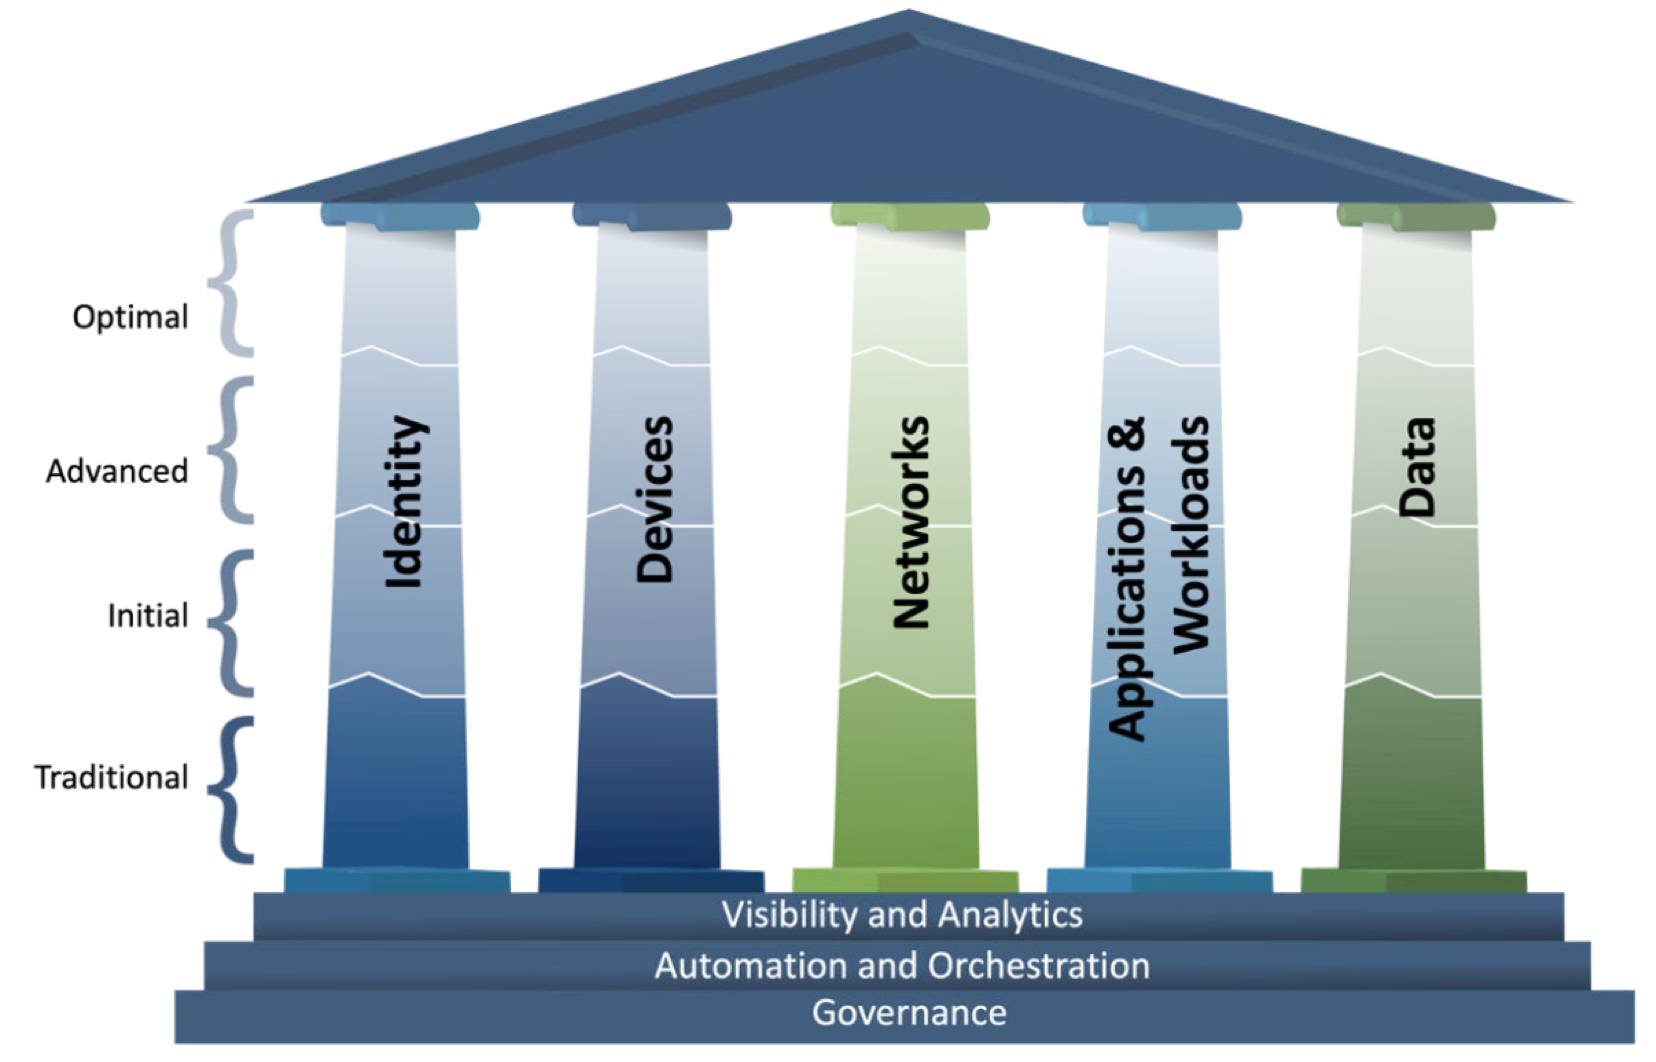
\includegraphics[width=0.9\textwidth]{images/ZTAPillars.png}
    \caption{5 trụ cột của ZTA theo NIST 800 - 207}
    \label{fig:ZTAPillars}
\end{figure}


\subsection{Ba hướng triển khai theo NIST}

Theo tài liệu của NIST \cite[tr. 12--14]{nist800207}, ZTA có thể được triển khai qua ba hướng tiếp cận chính:
\begin{itemize}
    \item \textbf{Enhanced Identity Governance (Quản trị danh tính nâng cao):} Sử dụng danh tính làm thành phần cốt lõi để tạo chính sách. Quyền truy cập vào tài nguyên được cấp dựa trên danh tính và các thuộc tính được gán cho chủ thể đó, trong khi mạng có thể vẫn mở cho mọi kết nối ban đầu.
    \item \textbf{Micro-segmentation (Phân khúc vi mô):} Chống lại kiến trúc mạng ``phẳng'' bằng cách sử dụng tường lửa hoặc cổng thông minh để chia mạng thành các phân đoạn rất nhỏ bao quanh từng tài nguyên hoặc nhóm tài nguyên. Cách này cô lập rủi ro và ngăn chặn triệt để sự di chuyển ngang của kẻ tấn công.
    \item \textbf{Software Defined Perimeter (Chu vi xác định bằng phần mềm - SDP):} Dựa trên cơ sở hạ tầng mạng (thường là mạng lớp 7) để quản lý luồng. Một bộ điều khiển mạng (\textit{Network Controller}) sẽ động thiết lập và cấu hình các đường truyền an toàn giữa máy khách và tài nguyên dựa trên quyết định từ Động cơ chính sách.
\end{itemize}

\subsection{So sánh ZTA với mô hình Perimeter-based Security}

Sự khác biệt giữa Kiến trúc Zero Trust và Mô hình bảo mật vành đai truyền thống được thể hiện rõ rệt qua cách tiếp cận với sự tin cậy và quyền truy cập (Bảng \ref{tab:zta_vs_perimeter}). Mô hình ZTA khắc phục triệt để các lỗ hổng của kiến trúc cũ, đặc biệt trong việc ngăn ngừa tấn công dịch chuyển ngang.

\begin{table}[htbp]
\centering
\caption{So sánh Mô hình bảo mật vành đai và Kiến trúc Zero Trust}
\label{tab:zta_vs_perimeter}
\begin{tabularx}{\textwidth}{|l|X|X|}
\hline
\rowcolor[HTML]{EFEFEF}
\textbf{Tiêu chí} & \textbf{Mô hình vành đai (Perimeter-based)} & \textbf{Kiến trúc Zero Trust (ZTA)} \\ \hline
\textbf{Giả định tin cậy} & Tin tưởng mặc định mọi thực thể bên trong mạng nội bộ. & Không tin tưởng bất kỳ thực thể nào, bất kể vị trí vật lý hay vị trí mạng. \\ \hline
\textbf{Cơ chế xác thực} & Xác thực tĩnh một lần tại thời điểm đăng nhập (tại cổng vào). & Đánh giá rủi ro động, xác thực liên tục và cấp quyền theo từng phiên giao dịch. \\ \hline
\textbf{Quyết định truy cập} & Dựa vào các thông tin tĩnh (ví dụ: địa chỉ IP, dải mạng). & Dựa trên danh tính xác thực mạnh, bối cảnh môi trường và mức độ rủi ro của thiết bị. \\ \hline
\textbf{Chống dịch chuyển ngang} & Vô cùng yếu kém. Tin tặc dễ dàng di chuyển khi đã thâm nhập thành công. & Vô hiệu hóa thành công nhờ xác thực độc lập từng tài nguyên và phân đoạn mạng vi mô. \\ \hline
\end{tabularx}
\end{table}